\section{Estructura}
En esta sección se detalla la estructura de todos los componentes de software de OpenGlove, los cuales son: el software de control Arduino, la API de bajo nivel C\#, las APIs de alto nivel  y la aplicación de configuración.





\subsection{Software de control Arduino}
La estructura del sofware de control Arduino corresponde a la desarrollada por \cite{tesis-cerda-rodrigo}, esta estructura se mantiene para este proyecto. En este trabajo se agrega el soporte a una nueva función que envía la versión actual del Sofware de configuración, siguiendo el versionamiento semántico propuesto por \cite{semantic-versioning-tom-preston-werner-coFounder-GitHub}. A continuación se muestra la forma de aplicar este versionamiento de manera resumida:

``Dado un número de versión MAJOR.MINOR.PATCH incrementar
\begin{itemize}
\item MAJOR cuando se tienen cambios incompatibles en la API
\item MINOR cuando se agrega funcionalidad compatible con anteriores versiones, y
\item PATCH cuando se hacen correcciones de errores compatibles con versiones anteriores.
\end{itemize}
El uso de etiquetas adicionales para pre-lanzamientos y metadatos, son extensiones al formato MAJOR.MINOR.PATCH." \citep{semantic-versioning-tom-preston-werner-coFounder-GitHub}. 

La versión utilizada para el software de control modificada es 1.1.0, considerando la versión de \cite{tesis-cerda-rodrigo} como versión 1.0.0 estable del software de control, dado que contiene todas las funcionalidades para administrar actuadores, flexores e IMU de la placa. La Figura \ref{fig:arduino-software-control} muestra la estructura del software de control, donde se aprecia que OpenGloveArduino es el código principal y que FunctionsSwitch contiene todas las funciones relativas a la placa y a los componentes de hardware conectados a ella (actuadores, flexores e IMU). La Tabla \ref{table:arduino-software-control} contiene la descripción del software de control.

\begin{figure}[H]
  \begin{center} 
   	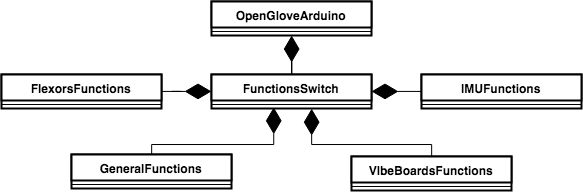
\includegraphics[width=1.0\textwidth]{images/chapter04/OpenGlove-Architecture-Arduino-Software.png} 
    \caption[Estructura del software de control Arduino]{Estructura del software de control Arduino \\Fuente: Elaboración propia (2018)}
    \label{fig:arduino-software-control}
  \end{center}
\end{figure}

%\caption[Descripción de la estructura software de control Arduino]{Descripción estructura del software de control Arduino \\Fuente: Elaboración propia (2018)}
%\label{table:arduino-software-control}

\begin{table}[H]
\centering
\caption[Descripción de la estructura software de control Arduino]{Descripción estructura del software de control Arduino \\Fuente: Elaboración propia (2018)}
\label{table:arduino-software-control}
\begin{tabular}{|l|l|l|l|}
\hline
Nombre             & Descripción                                                                                                                                                                                                                                                                                                                                                                                                                                 & Origen                                                    & Estado Actual                                           \\ \hline
OpenGloveArduino   & \begin{tabular}[c]{@{}l@{}}"Contiene el código principal de Arduino,\\ desde el cual se realizan los llamados\\ de las funciones disponibles en\\ FunctionsSwitch.  Algunas de éstas son\\ invocadas solo cuando  hay datos \\ disponibles, mientras que las funciones\\ que requieren un llamado constante como\\ las dedicadas a la lectura de un sensor,\\ son llamadassin necesidad de datos\\ entrantes" (Cerda, 2017).\end{tabular} & \begin{tabular}[c]{@{}l@{}}Cerda\\ (2017)\end{tabular}    & Modificado                                              \\ \hline
FunctionsSwitch    & \begin{tabular}[c]{@{}l@{}}"Se encarga de evaluar e invocar el tipo\\ defunción  solicitada, con el fin de\\ realizar cambios en la  instancia de la\\ biblioteca correspondiente a dicha\\ función"(Cerda, 2017).\end{tabular}                                                                                                                                                                                                           & \begin{tabular}[c]{@{}l@{}}Cerda\\ (2017)\end{tabular}    & \begin{tabular}[c]{@{}l@{}}Sin\\ modificar\end{tabular} \\ \hline
GeneralFunctions   & \begin{tabular}[c]{@{}l@{}}Contiene las funciones generales de\\ Arduino (lecturas/escrituras y\\ digitales/análogas). Se  destaca la función\\ setLoopDelay() para definir el retraso\\ de los ciclos de la placa\\ en milisegundos. Por defecto es 60 ms,\\ por tanto para obtener la mayor velocidad\\ de la placa Arduino, se debe utilizar la\\ función  SetLoopDelay disponible en la\\ API de alto nivel.\end{tabular}               & \begin{tabular}[c]{@{}l@{}}Monsalve\\ (2015)\end{tabular} & \begin{tabular}[c]{@{}l@{}}Sin\\ modificar\end{tabular} \\ \hline
FlexorsFunctions   & \begin{tabular}[c]{@{}l@{}}"Contiene todas las variables y funciones\\ necesarias para representar los flexores \\ del guante y su configuración." (Cerda, 2017).\\ Si se requiere aumentar la cantidad máxima\\ de flexores por placa (10) debe realizarse a\\ nivel del software de control Arduino.\end{tabular}                                                                                                                        & \begin{tabular}[c]{@{}l@{}}Cerda\\ (2017)\end{tabular}    & \begin{tabular}[c]{@{}l@{}}Sin\\ modificar\end{tabular} \\ \hline
VibeBoardFunctions & \begin{tabular}[c]{@{}l@{}}Contiene todas las funciones necesarias para\\ inicializar, activar y desactivar los actuadores.\end{tabular}                                                                                                                                                                                                                                                                                                    & \begin{tabular}[c]{@{}l@{}}Monsalve\\ (2015)\end{tabular} & \begin{tabular}[c]{@{}l@{}}Sin\\ modificar\end{tabular} \\ \hline
ImuFunctions       & \begin{tabular}[c]{@{}l@{}}"Contiene todas las variables y funciones\\ necesarias para el funcionamiento y\\ configuración del sensor de rastreo \\ IMU." (Cerda, 2017).\end{tabular}                                                                                                                                                                                                                                                      & \begin{tabular}[c]{@{}l@{}}Cerda\\ (2017)\end{tabular}    & \begin{tabular}[c]{@{}l@{}}Sin\\ modificar\end{tabular} \\ \hline
\end{tabular}
\end{table}







\subsection{API C\# de bajo nivel}
Redactando ...

\begin{figure}[H]
  \begin{center} 
   	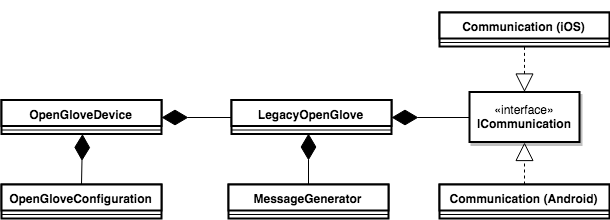
\includegraphics[width=1.0\textwidth]{images/chapter04/OpenGlove-Architecture-API-CSharp-LowLevel.png} 
    \caption[Diagrama de clases API C\# de bajo nivel]{Diagrama de clases API C\# de bajo nivel \\Fuente: Elaboración propia (2018)}
    \label{fig:api-csharp-ll}
  \end{center}
\end{figure}


%\caption[Descripción del diagrama de clases API C\# de bajo nivel]{Descripción del diagrama de clases API C\# de bajo nivel \\Fuente: Elaboración propia (2018)}
%\label{table:api-csharp-ll}


\begin{table}[H]
\centering
\caption[Descripción del diagrama de clases API C\# de bajo nivel]{Descripción del diagrama de clases API C\# de bajo nivel \\Fuente: Elaboración propia (2018)}
\label{table:api-csharp-ll}
\begin{tabular}{|l|l|l|l|}
\hline
Nombre                                                             & Descripción                                                                                                                                                                                                                                                                                                                                                                                                                                                                                                                                                    & Origen                                                 & Estado Actual                                                                                           \\ \hline
OpenGloveDevice                                                    & \begin{tabular}[c]{@{}l@{}}Clase que representa un dispositivo OpenGlove,\\ la cual incluye su identificación, configuración y\\ todos los métodos que permiten la comunicación\\ con el software de control Arduino y la inicializa-\\ ción de la configuración en la placa Arduino.\end{tabular}                                                                                                                                                                                                                                                             & Nuevo                                                  & Completado                                                                                              \\ \hline
\begin{tabular}[c]{@{}l@{}}OpenGloveConfi-\\ guration\end{tabular} & \begin{tabular}[c]{@{}l@{}}Representa la configuración global de un\\ dispositivo OpenGlove. Esta incluye la\\ configuración de la placa Arduino, el mapeo de\\ actuadores, el mapeo de flexores y la configuración\\ del IMU. Dicha configuración global puede estar\\ o no inicializada en el dispositivo físico.\end{tabular}                                                                                                                                                                                                                               & Nuevo                                                  & Completado                                                                                              \\ \hline
LegacyOpenGlove                                                    & \begin{tabular}[c]{@{}l@{}}Clase que representa la API C\# de bajo nivel\\ desarrollada por Monsalve (2015) y Cerda (2017),\\ modificada para obtener la versión del software\\ de control Arduino.\end{tabular}                                                                                                                                                                                                                                                                                                                                               & \begin{tabular}[c]{@{}l@{}}Cerda\\ (2017)\end{tabular} & Modificado                                                                                              \\ \hline
MessageGenerator                                                   & \begin{tabular}[c]{@{}l@{}}Clase que permite la generación de mensajes\\ bajo el protocolo establecido por Monsalve (2015)\\ para los actuadores y la extensión realizada por\\ Cerda (2017) para dar soporte a los flexores e\\ IMU. Esta clase fue modificada para obtener\\ la versión del software de control Arduino.\end{tabular}                                                                                                                                                                                                                        & \begin{tabular}[c]{@{}l@{}}Cerda\\ (2017)\end{tabular} & Modificado                                                                                              \\ \hline
ICommunication                                                     & \begin{tabular}[c]{@{}l@{}}Interfaz que contiene la definición de métodos que\\ deben ser implementados para obtener: la lista de\\ dispositivos emparejados, la conexión/desconexión\\ de los mismos y la escritura/lectura de mensajes. \\ Esta interfaz debe ser implementada en cada\\ sistema operativo que desee utilizar OpenGlove,\\ para ello se debe consultar las plataformas\\ soportadas por Xamarin.Forms, este proyecto\\ incluye el soporte para Android.\end{tabular}                                                                         & Nuevo                                                  & Completado                                                                                              \\ \hline
\begin{tabular}[c]{@{}l@{}}Communication\\ (Android)\end{tabular}  & \begin{tabular}[c]{@{}l@{}}Implementación de la interfaz ICommunication\\ en el proyecto Android de Xamarin.Forms. Hace\\ uso de las APIs Bluetooth de Android\\ permitiendo obtener la lista de dispositivos\\ emparejados, la conexión/desconexión de\\ dispositivos y la escritura/lectura del socket\\ Bluetooth creado. Esta clase crea un hilo que\\ administra cada conexión Bluetooth de manera\\ independiente, este hilo permite que otros objetos\\ se suscriban para recibir los mensajes que envie\\ el software de control Arduino.\end{tabular} & Nuevo                                                  & Completado                                                                                              \\ \hline
\begin{tabular}[c]{@{}l@{}}Communication\\ (iOS)\end{tabular}      & \begin{tabular}[c]{@{}l@{}}Implementación de la interfaz\\ ICommunication en el proyecto iOS de\\ Xamarin.Forms. Los métodos de esta clase\\ arrojan la excepción NotImplementedException.\\ Es necesario implementar los métodos de esta\\ clase para dar soporte a OpenGlove en iOS, para\\ ello debe utilizarse un dispositivo físico.\end{tabular}                                                                                                                                                                                                         & Nuevo                                                  & \begin{tabular}[c]{@{}l@{}}Incompleto,\\ se requiere\\ implementar \\ los métodos\\ en iOS\end{tabular} \\ \hline
\end{tabular}
\end{table}




\subsection{API C\# alto nivel}
Redactando ...

\begin{figure}[H]
  \begin{center} 
   	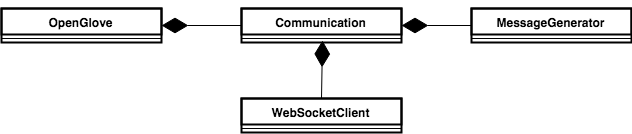
\includegraphics[width=1.0\textwidth]{images/chapter04/OpenGlove-Architecture-API-CSharp-HL.png} 
    \caption[Diagrama de clases API C\# de alto nivel]{Diagrama de clases API C\# de alto nivel \\Fuente: Elaboración propia (2018)}
    \label{fig:api-csharp-hl}
  \end{center}
\end{figure}


%\caption[Descripción del diagrama de clases API C\# de alto nivel]{Descripción del diagrama de clases API C\# de alto nivel \\Fuente: Elaboración propia (2018)}
%\label{fig:api-csharp-hl}





\subsection{API Java alto nivel}
Redactando ...

\begin{figure}[H]
  \begin{center} 
   	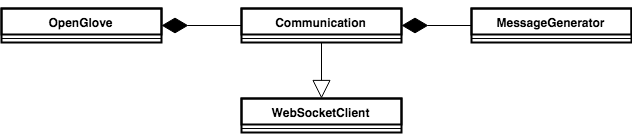
\includegraphics[width=1.0\textwidth]{images/chapter04/OpenGlove-Architecture-API-Java-HL.png} 
    \caption[Diagrama de clases API Java de alto nivel]{Diagrama de clases API Java de alto nivel \\Fuente: Elaboración propia (2018)}
    \label{fig:api-java-hl}
  \end{center}
\end{figure}




\subsection{Aplicación de configuración}
Redactando ... 

\begin{figure}[H]
  \begin{center} 
   	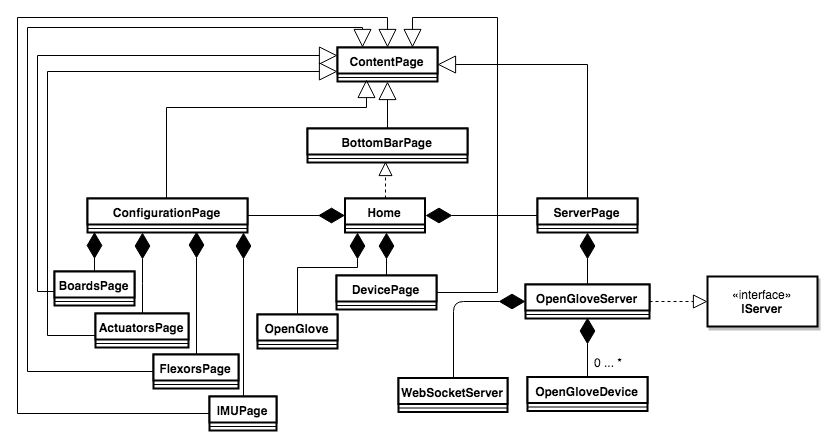
\includegraphics[width=1.0\textwidth]{images/chapter04/OpenGlove-Architecture-Configuration-App.png} 
    \caption[Diagrama de clases aplicación de configuración]{Diagrama de clases aplicación de configuración \\Fuente: Elaboración propia (2018)}
    \label{fig:class-diagram-configuarion-app}
  \end{center}
\end{figure}
